\section{Design}
\label{sec:design}

In this section, we introduce the system design of \sys. We begin by presenting the data structure employed in \sys and demonstrate how Block-Sparse Row (BSR) acts as a versatile abstraction for KV cache storage in attention kernels. Next, we discuss the \sys compiler, which supports various attention variants, alongside a dynamic-aware runtime scheduler that facilitates load-balanced scheduling of attention kernels. Finally, we describe the user-level API designed for integrating \sys with existing LLM serving systems.

\subsection{KV-Cache Storage}

\subsubsection{Block-Sparse Matrix as Unified Format}

Recent advancements in KV-Cache storage, such as PageAttention~\cite{kwon2023vllm} and RadixAttention~\cite{zheng2023sglang}, employ non-contiguous memory storage with a minimum granularity of a block (or token) of $(H, D)$ tensors, where $H$ represents the number of heads and $D$ the hidden dimension. These structures are optimized to minimize memory fragmentation while enhancing memory reuse and cache hit rates. We demonstrate that these diverse data structures can be unified under a block sparse format, as illustrated in Figure~\ref{fig:focus-sparse-layout}.

\begin{figure}[ht]
    \centering
    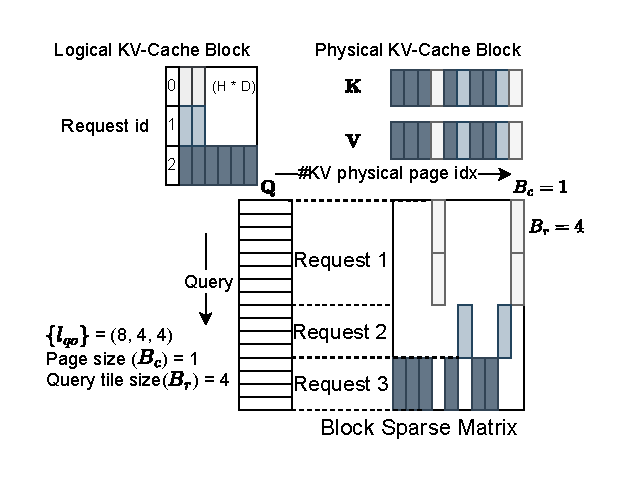
\includegraphics[width=0.45\textwidth]{figures/flashinfer-sparsetir-format.pdf}
    \caption{Representation of Page Table in BSR $(B_r=4,B_c=1)$ format. The number of column blocks in the block sparse matrix corresponds to the total number of blocks allocated for the Page Table. Non-zero blocks represent KV-Cache pages accessed by queries.}
    \label{fig:focus-sparse-layout}
\end{figure}

The conceptual equivalence between page tables and sparse matrices has been previously explored in SPGrid~\cite{setaluri2014spgrid}, which leverages Translation Lookaside Buffer (TLB) hardware for efficient sparse structure indexing. Beyond page tables and radix trees, sparse matrices can also effectively represent various attention mechanisms, such as Tree Attentions used in speculative decoding~\cite{cai2024medusa,miao2023specinfer,chen2024sequoia} and importance masks applied to KV-Cache~\cite{tang2024quest}.

In \sys, we implement a unified strategy for data representation. Query and output matrices are efficiently stored as ragged tensors (also known as jagged arrays)~\cite{ragged-tensor} without padding, which facilitates the compact packing of queries and outputs from diverse requests into a single tensor. Initially, keys and values are maintained in ragged tensors using the same index pointers as queries, as they originate from the projection matrices $W_q, W_k, W_v$ applied to the same input. These keys and values are subsequently incorporated into the KV-Cache with newly updated entries. The KV-Cache employs a block-sparse row (BSR) format, where block sizes are defined by application requirements: $B_r$ corresponds to the query tile size, details of which will be discussed in later sections, and $B_c$ is specified by KV-Cache management algorithms. \sys kernel implementations supports arbitrary $(B_r, B_c)$ values.

\begin{figure}[ht]
    \centering
    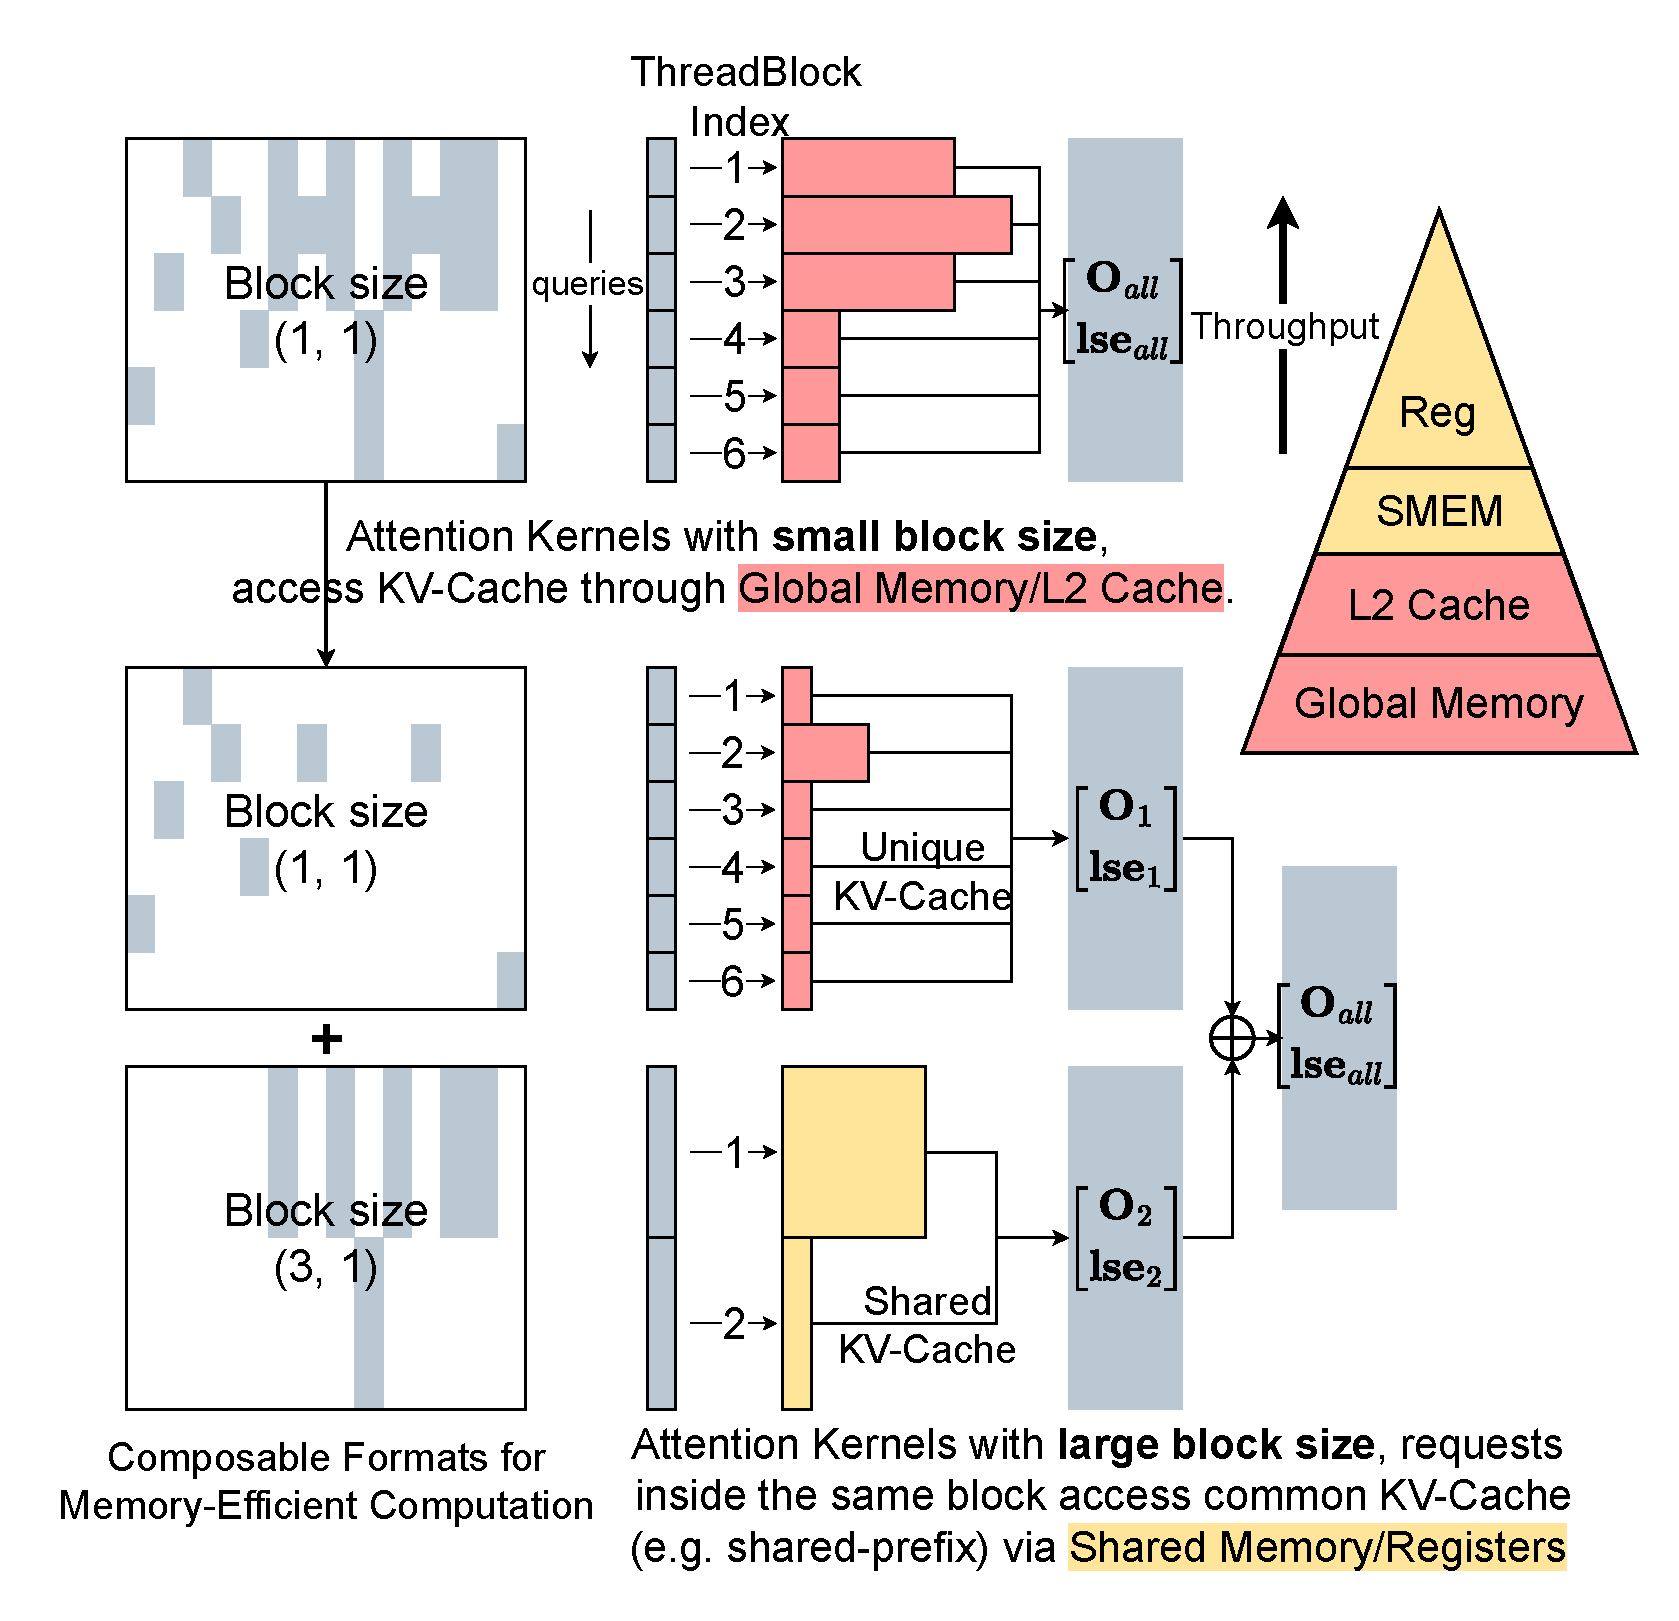
\includegraphics[width=0.45\textwidth]{figures/flashinfer-composable-formats.pdf}
    \caption{Composable formats for shared-prefix decomposition in attention computation. The queries corresponding to the first 6 rows have a shared prefix, as do the queries in the last 6 rows. We store the KV cache corresponding to the shared prefix in a block sparse matrix with a block size of $(3,1)$, while storing the remaining unique KV cache in another block sparse matrix with a block size of $(1,1)$. For block size $(3,1)$, 3 queries can share the same KV cache in high-bandwidth shared memory, while for block size $(1,1)$, each query access KV-Cache within its own threadblock, which can only go through low-bandwidth global memory or L2 cache.}
    \label{fig:flashinfer-composable-formats}
\end{figure}
\subsubsection{Composable Formats for Memory Efficiency}
\label{sec:composable-formats}

Inspired by SparseTIR~\cite{ye2023sparsetir}, we enhance attention computation efficiency through composable formats. This approach leverages multiple block sparse formats instead of a single format to store the sparse matrix, offering greater flexibility and memory efficiency. Single block-sparse formats are constrained by a fixed block size, limiting memory efficiency based on the number of rows in the block ($B_r$). While larger $B_r$ values improve shared memory and register reuse for requests within the same block, they also increase fragmentation. Conversely, requests in different blocks cannot access each other's shared memory.

Our composable format design allows for the decomposition of the KV cache sparse matrix based on prior knowledge. For instance, if certain requests share a prefix, the corresponding rows and columns in the KV cache form a dense submatrix. We can then use a block sparse matrix with a larger $B_r$ to store these submatrices efficiently. Figure~\ref{fig:flashinfer-composable-formats} illustrates this concept, showing how shared prefixes can be optimized using composable formats. This approach doesn't require data movement in the KV cache; instead, we compute the indices and index pointer arrays for the sparse submatrices. Attention computations on larger block sizes can access shared KV cache entries using fast shared memory and registers, significantly improving memory efficiency.

\subsection{Compute Abstraction}
\label{sec:compute-abs}

We developed CUDA/CUTLASS \cite{cutlass} templates for FlashAttention, designed specifically for both dense and block-sparse matrices and compatible with NVIDIA GPU architectures from Turing to Hopper (sm75 to sm90a). Our implementations utilize the FlashAttention2 (FA2 for short) algorithm \cite{dao2023flashattention2} for architectures up to Ada(sm89), and the FlashAttention3 (FA3 for short) algorithm \cite{jay2024flashattention3} for Hopper. Key improvements include enhanced loading of sparse tiles into shared memory, expanded tile-size configurations, optimized memory access patterns for grouped query attention, and customizable attention variants.

\subsubsection{Global to Shared Memory Data Movement}
\label{sec:sparse-loading}

The \sys attention template supports any block size, requiring a specialized data loading approach since blocks may not align with tensor core shapes. As discussed in Section \ref{sec:block-sparse}, we address these challenges by transferring tiles from scattered global memory to contiguous shared memory for dense tensor core operations. Tensor core inputs for a single MMA instruction can originate from different blocks within a block-sparse matrix. Figure \ref{fig:sparse-loading} illustrates how \sys loads tiles from sparse/dense KV-Cache into shared memory; sparse KV-Cache addresses are computed using the \texttt{indices} arrays of the BSR matrix, while dense ones use row index affine transformations.

The last dimension of the KV-Cache remains contiguous (with size of head dimension $d$, commonly 128 or 256), maintaining coalesced memory access that fits GPU cache line sizes. We use asynchronous copy instructions \texttt{LDGSTS} with a 128B width to maximize memory bandwidth. Although the Tensor Memory Accelerator (TMA) in Hopper architecture can further accelerate data movement, it doesn't support non-affine memory access patterns. Consequently, we only use TMA for contiguous KV-Cache on Hopper GPUs and fall back to Ampere-style asynchronous copies for other settings where TMA isn't suitable.

\begin{figure}[ht]
    \centering
    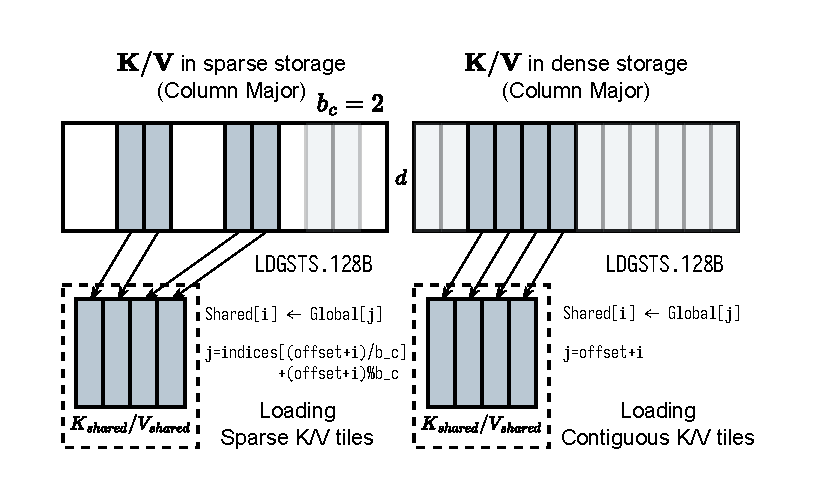
\includegraphics[width=0.45\textwidth]{figures/flashinfer-sparse-loading.pdf} 
    \caption{Data transfer from global to shared memory for sparse/dense KV-Cache in \sys. Left: Sparse KV-Cache with $b_c=2$; Right: Dense KV-Cache. Head dimension $d$.}
    \label{fig:sparse-loading}
\end{figure}

Post-transfer to shared memory, the sparse and dense FlashAttention implementations converge, allowing consistent kernel usage with variations only in data loading modules.

\subsubsection{Microkernel with Different Tile Sizes}
\label{sec:tile-size-selection}

To adapt to the varying operational intensities of LLM applications, \sys implements the FA2 algorithm across multiple sizes. Traditional FA2 uses limited number of tile sizes (e.g., $(128,64)$), optimal for prefill on A100 but inefficient for shorter-query-length decoding. One architecture's ideal tile size may not suit others; for instance, Ada(sm89) has limited shared memory, affecting SM occupancy with large tiles.

\sys offers FA2 kernels with tile sizes ${(1, 16, 32, 64, 128) \times (32, 64, 128)}$ and selects using heuristics based on hardware resources and workload intensity:

\begin{enumerate}[itemsep=2pt,topsep=0pt,parsep=0pt]
\item Determine average query length (for Grouped-Query Attention, the query length are fused with head group dimension, see Appendix \ref{sec:head-group-fusion}) per batch, choosing the minimal query tile size meeting or exceeding it.
\item Formulate register and shared memory constraints as functions of K/V tile size, maximizing SM resource occupancy.
\end{enumerate}

\begin{figure*}[!ht]
    \centering
    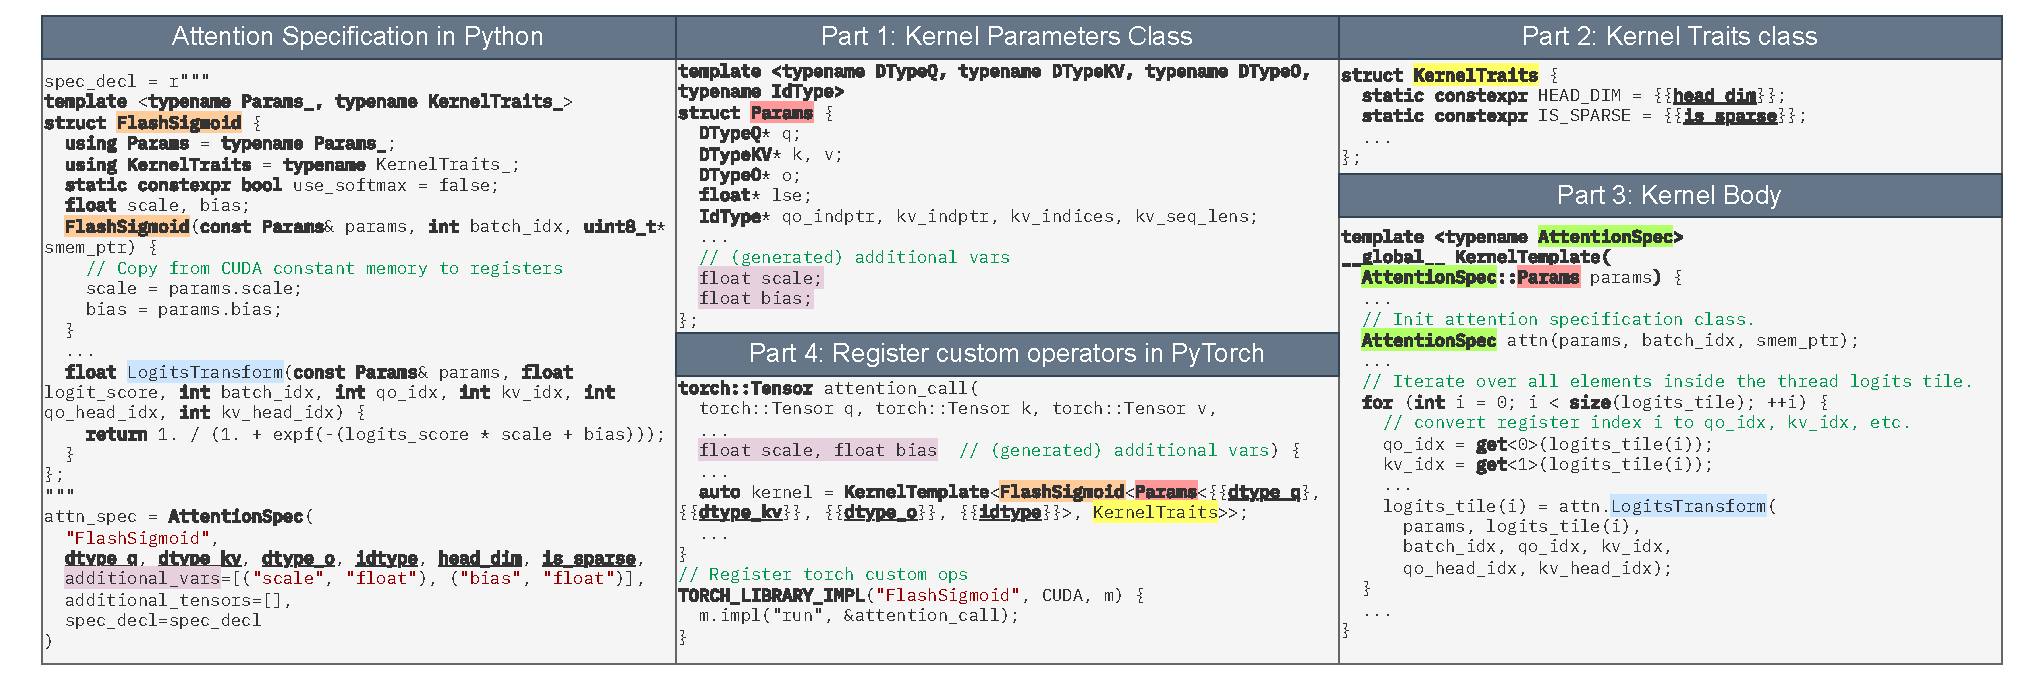
\includegraphics[width=1\textwidth]{figures/flashinfer-jit.pdf}
    \caption{JIT compiler for attention variants in \sys, featuring CUDA code strings defining variant functors, additional variables/tensors, and data types, used to populate kernel templates. Corresponding codes share highlighting.}
    \label{fig:flashinfer-attention-variants}
\end{figure*}
\subsubsection{JIT Compiler for Attention Variants}


For query tile size $1$, we use CUDA Cores template since tensor core instruction $m$ (minimum rows) is $16$, and use Tensor Cores for other query tile sizes. For FA3 we provides row tile sizes that are multiples of $64$, aligning with  Hopper's WGMMA requirements. Tile sizes resolve at compile-time considering task specifics (decoding, prefill, etc.) and hardware capabilities. The block row size $B_r$ is block-sparse matrix is aligned with the query tile size $T_q$.

Recent LLM models use variants to standard attention algorithms. Supporting various attention variants in CUDA library is not sustainable because the we specialize the kernel for each variant for maximum performance, and the number of variants is growing rapidly. However, most attention variants have similar structure to the vanilla attention so we can use the same skeleton of FlashAttention kernels with small modifications. Inspired by FlexAttention ~\cite{he2024flexattention}, we designed a customizable CUDA template and a JIT compiler that takes the attention variant specification as input and generates the optimized kernel code. The variant specification includes the following functors:

\begin{itemize}[itemsep=2pt,topsep=0pt,parsep=0pt]
    \item \texttt{QueryTransform, KeyTransform, ValueTransform}: The transformation applied to the query/key/value tensor before the attention computation.
    \item \texttt{OutputTransform}: The transformation applied to the attention output tensor before returning.
    \item \texttt{LogitsTransform, LogitsMask}: The transformation applied to the logits tensor before the softmax computation, and the mask applied to the logits tensor.
\end{itemize}

Each functor has a fixed signature that takes the kernel parameters, input and current query/key/head index as input, and returns the output. Those variant functions are specified as member of a user-defined variant class which creates a closure for the variant functors. Functors such as \texttt{LogitsTransform} and \texttt{LogitsMask} are inspired by FlexAttention ~\cite{he2024flexattention} and can be used to implement the attention variants with customized logits postprocessing such as custom mask, logits soft-cap ~\cite{morgane2024gemma2,grok} and sliding window attention ~\cite{beltagy020longformer}. \sys has an option of using softmax or not in the attention variant specification, which makes it capable of supporting attention variants that don't use softmax, such as FlashSigmoid ~\cite{jason2024flashsigmoid}. \sys's query and key transformation functors making it possible to fuse normalization, RoPE ~\cite{su2024rope} and projection ~\cite{deepseekv2} into the attention kernel.

Figure \ref{fig:flashinfer-attention-variants} shows how \sys maps FlashSigmoid's ~\cite{jason2024flashsigmoid} attention specification to different parts of \sys's CUDA templates. Attention specificiation accepts a piece of CUDA code to define the variant functors, such design also enables user to use advanced PTX instructions \footnote{\url{https://docs.nvidia.com/cuda/parallel-thread-execution/}} or even their own libraries. The JIT compiler generates the CUDA code by inserting the variant class and other information into the template, and the generated CUDA code is compiled with PyTorch's JIT compiler \footnote{\url{https://pytorch.org/tutorials/advanced/cpp_extension.html\#jit-compiling-extensions}} and registered as a custom operator \footnote{\url{https://pytorch.org/tutorials/advanced/custom_ops_landing_page.html}}. We also support compiling to other runtime systems through a framework agnostic DLPack \footnote{\url{https://github.com/dmlc/dlpack}} interface.

\subsection{Dynamism-Aware Runtime}

In this section we introduce the runtime design of \sys, including the dynamic scheduling framework, and the composable formats for memory efficient attention.

\subsubsection{Load-balanced Scheduling}

\label{sec:load-balanced-scheduling}

In \sys, the load-balanced scheduling algorithm aims to minimize SM idle time by distributing the workload evenly across all SMs. It takes the sequence length information of the query/output and key/value dimensions as input, and produces both the mapping between the workload and Cooperative Thread Arrays (CTAs) and the index mapping for partial and final outputs. The algorithm is presented in Algorithm~\ref{alg:load-balancing} (the head dimension is omitted for simplicity). Our approach is inspired by Stream-K~\cite{osama2023streamk}; however, because LLM serving requires deterministic outputs, we did not incorporate atomic aggregation in Stream-K implementation to avoid non-deterministic behavior. The scheduling algorithm generates deterministic aggregation order when provided with identical sequence length information.
\begin{algorithm}[tb]
   \scriptsize
   \caption{\sys's balanced scheduling algorithm}
   \label{alg:load-balancing}
\begin{algorithmic}[1]
   \STATE {\bfseries Input:} $\{l_{qo}(i), l_{kv}(i)\}_i$, query tile size $T_q$.
   \STATE Define the cost of a tile $l_q, l_{kv}$ as ($\alpha, \beta$ are hyperparameters):
   $$\textrm{cost}(l_q, l_{kv}) = \alpha l_q + \beta l_{kv} $$
   \STATE Compute the maximum KV chunk size $L_{kv}$ by
   \vspace{-1em}
   $$L_{kv} \leftarrow \frac{\sum_{i}\ceil{\frac{l_{qo}(i)}{T_q}}\cdot l_{kv}(i)}{\#\textrm{CTA}}$$
   \STATE Split each query tile's KV into chunks, with maximum size $L_{kv}$, we assign each chunk a work index $w$, and the length of the chunk is $l_{kv}(w)$.
   \STATE Let $W = \{(w, l_{kv}(w))\}$ and sort the entries in descending order of length.
   \STATE $Q \leftarrow \textrm{PriorityQueue}(\{(c, 0)\})$ where $c$ is the CTA index.
   \WHILE{$W \neq \emptyset$}
      \STATE $c, \textrm{current\_cost} \leftarrow Q.\textrm{pop}_{min}()$
      \STATE $w, l_{kv}(w) \leftarrow W.\textrm{pop}()$
      \STATE $\textrm{new\_cost} \leftarrow \textrm{current\_cost} + \textrm{cost}(T_q, l_{kv}(w))$
      \STATE Assign chunk $w$ to CTA $c$
      \STATE $Q.\textrm{push}((c, \textrm{new\_cost}))$
   \ENDWHILE
\end{algorithmic}
   \normalsize
\end{algorithm}

Figure \ref{fig:flashinfer-scheduler} shows the workflow of \sys's runtime scheduler. The attention kernel do not produce the final output directly because some long KV are split into multiple chunks, and the final output is the contraction (using the attention composition operator mentioned in section \ref{sec:attention-composition}) of all chunks' partial outputs.
The partial outputs are stored in a workspace buffer provided by the user (see section \ref{sec:programming-interface}).
\sys implements efficient attention composition operator that can deal with variable length aggregation. The work queue of each CTA, and the mapping between partial and final outputs need to be planned by the scheduler. Once plan information is computed on CPU, \sys asynchronously copy the plan information to a specific region of the workspace buffer on GPU, and the plan information is used as inputs for persistent attention/contraction kernels. The scheduler runs per generation step to produce plan information as the sequence length changes for each generation step on CPU, and overhead can be amortized over multiple layers because the same plan information can be reused for all layers.

\begin{figure}[ht]
    \centering
    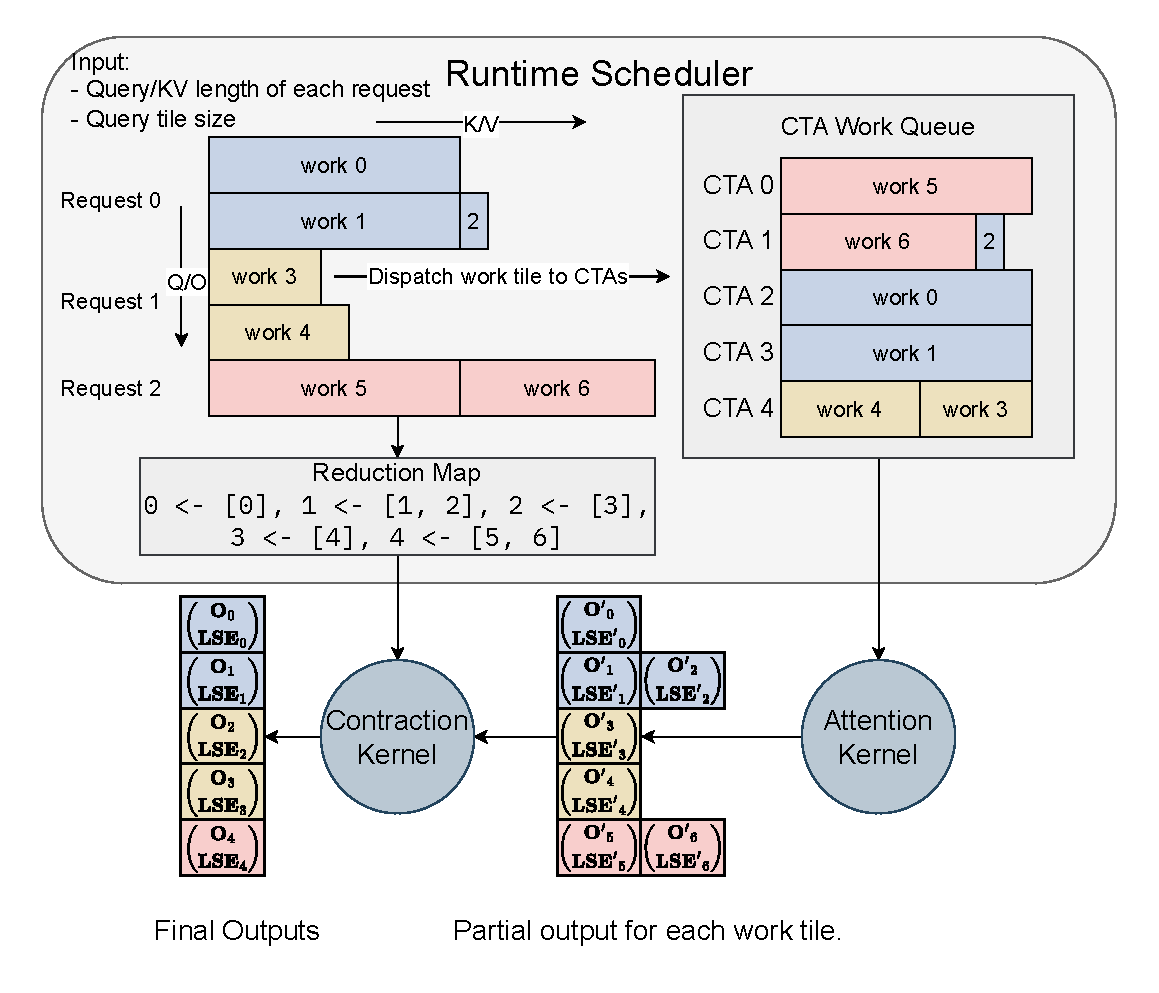
\includegraphics[width=0.4\textwidth]{figures/focus-scheduler.pdf}
    \caption{\sys's load-balanced runtime scheduler, sequence length information (both on query/output and key/value dimension) are provided to the scheduler to compute the plan information: (1) Work queue of each CTA (2) Index mapping between partial and final outputs. These plan information are cached at GPU-side and used as inputs for persistent attention/contraction kernels.}
    \centering
    \label{fig:flashinfer-scheduler}
\end{figure}

\sys guarantees both attention and contraction stage are compatible with CUDAGraphs ~\cite{alan2019cudagraph,vinh2021pytorchcudagraph}. Both attention and contraction stage use persistent kernel and the grid size is fixed once compiled, which means the kernel is launched with the same grid size for each generation step. We set the fixed offset for each section of the workspace buffer to store partial outputs and plan information to make sure the pointers passed to the kernel are the same for each generation step, meeting the requirement of CUDAGraphs (see Appendix \ref{sec:cudagraph-compatible-layout} for details). We merge the two stages into one persistent kernel, eliminating intra-kernel overhead.

\subsection{Programming Interface}
\label{sec:programming-interface}

\sys offers a programming interface designed for seamless integration with existing LLM serving frameworks such as vLLM\cite{kwon2023vllm}, MLC-Engine\cite{mlcllm}, and SGLang~\cite{zheng2023sglang}.

\lstinputlisting[style=zihao-style, morekeywords={with}, label={lst:programming-interface}, caption={\sys PyTorch Programming Interface}]{code/programming_interface.py}

Listing \ref{lst:programming-interface} shows the PyTorch programming interface of \sys. The user initializes the wrapper by providing the attention variant specification, task information, and a user-allocated workspace buffer (see Appendix \ref{sec:memory-mgmt} for details) to store partial output and plan information for \sys dynamic scheduling.
Kernel are JIT-compiled at init time and cached for reuse. For composable formats (section \ref{sec:composable-formats}), \sys creates multiple attention wrappers, each with distinct block sizes. Kernels with different average query length and composable format configurations are compiled and captured in different CUDAGraphs. At runtime, the serving framework selects the most appropriate CUDAGraph based on the current KV-Cache configuration, ensuring optimal performance for varying workload characteristics.

The \texttt{plan} function activates the dynamic scheduler by processing sequence length data to generate load-balanced scheduling plans. These plans are cacheable, allowing reuse across operators with matching sequence length specs, such as all decode attentions in a generation step. The \texttt{run} function executes the attention computation using inputs of query, key, value, and cached plan data, outputting the attention results. 
CUDAGraph can capture calls to \texttt{run} functions and compile the entire attention generation step into a single graph. However, \texttt{plan} function is not captured by CUDAGraph because it's on CPU. The \texttt{plan} and \texttt{run} division is inspired by the Inspector-Executor (IE) model \cite{ravi1988principles, saltz1991preprocessed, ravi1993runtime},  which is widely used for parallelizing irregular workloads.
